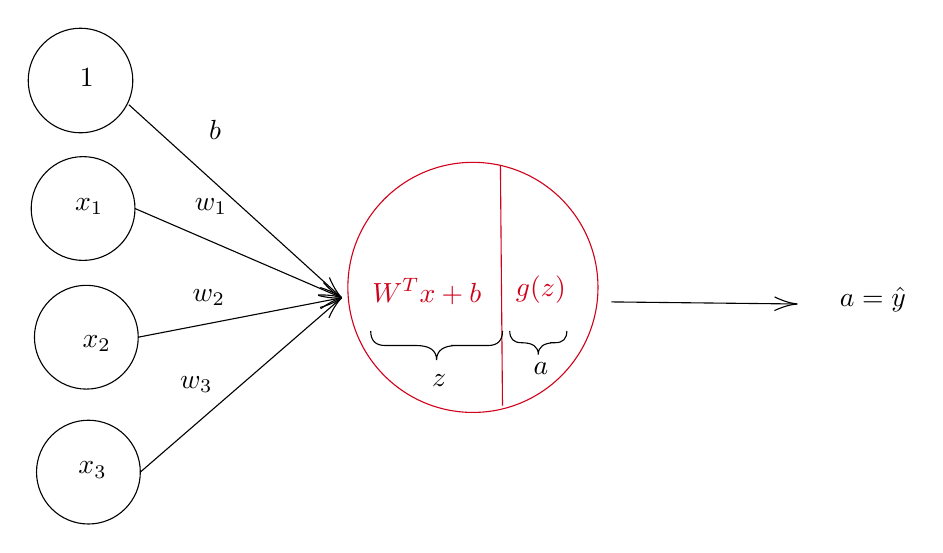
\begin{tikzpicture}[x=0.75pt,y=0.75pt,yscale=-1,xscale=1]
%uncomment if require: \path (0,300); %set diagram left start at 0, and has height of 300

\draw    (101.43, 102) circle [x radius= 25, y radius= 25]  ;
\draw    (103, 164) circle [x radius= 25, y radius= 25]  ;
\draw    (104, 229) circle [x radius= 25, y radius= 25]  ;
\draw  [color={rgb, 255:red, 208; green, 2; blue, 27 }  ,draw opacity=1 ]  (289.25, 140) circle [x radius= 60.25, y radius= 60.25]  ;
\draw    (126.43,102) -- (226,145) ;
\draw [shift={(226,145)}, rotate = 203.36] [color={rgb, 255:red, 0; green, 0; blue, 0 }  ]   (0,0) .. controls (3.31,-0.3) and (6.95,-1.4) .. (10.93,-3.29)(0,0) .. controls (3.31,0.3) and (6.95,1.4) .. (10.93,3.29)   ;

\draw    (128,164) -- (226,145) ;
\draw [shift={(226,145)}, rotate = 529.03] [color={rgb, 255:red, 0; green, 0; blue, 0 }  ]   (0,0) .. controls (3.31,-0.3) and (6.95,-1.4) .. (10.93,-3.29)(0,0) .. controls (3.31,0.3) and (6.95,1.4) .. (10.93,3.29)   ;

\draw    (129,229) -- (226,145) ;
\draw [shift={(226,145)}, rotate = 499.11] [color={rgb, 255:red, 0; green, 0; blue, 0 }  ]   (0,0) .. controls (3.31,-0.3) and (6.95,-1.4) .. (10.93,-3.29)(0,0) .. controls (3.31,0.3) and (6.95,1.4) .. (10.93,3.29)   ;

\draw    (356,147) -- (445.5,148) ;
\draw [shift={(445.5,148)}, rotate = 180.64] [color={rgb, 255:red, 0; green, 0; blue, 0 }  ]   (0,0) .. controls (3.31,-0.3) and (6.95,-1.4) .. (10.93,-3.29)(0,0) .. controls (3.31,0.3) and (6.95,1.4) .. (10.93,3.29)   ;

\draw    (100.19, 40.33) circle [x radius= 25.19, y radius= 25.19]  ;
\draw    (123.5,52) -- (226,145) ;
\draw [shift={(226,145)}, rotate = 222.22] [color={rgb, 255:red, 0; green, 0; blue, 0 }  ]   (0,0) .. controls (3.31,-0.3) and (6.95,-1.4) .. (10.93,-3.29)(0,0) .. controls (3.31,0.3) and (6.95,1.4) .. (10.93,3.29)   ;

\draw [color={rgb, 255:red, 208; green, 2; blue, 27 }  ,draw opacity=1 ]   (302.5,81) -- (303.5,197) ;


\draw   (240,161) .. controls (240,165.67) and (242.33,168) .. (247,168) -- (261.75,168) .. controls (268.42,168) and (271.75,170.33) .. (271.75,175) .. controls (271.75,170.33) and (275.08,168) .. (281.75,168)(278.75,168) -- (296.5,168) .. controls (301.17,168) and (303.5,165.67) .. (303.5,161) ;
\draw   (307,161) .. controls (307,164.77) and (308.89,166.66) .. (312.66,166.66) -- (312.66,166.66) .. controls (318.05,166.66) and (320.75,168.55) .. (320.75,172.32) .. controls (320.75,168.55) and (323.45,166.66) .. (328.84,166.66)(326.41,166.66) -- (328.84,166.66) .. controls (332.61,166.66) and (334.5,164.77) .. (334.5,161) ;

\draw (108,167) node   {$x_{2}$};
\draw (104.37,100.96) node   {$x_{1}$};
\draw (106,228) node   {$x_{3}$};
\draw (103.21,38.84) node   {$1$};
\draw (165,64) node   {$b$};
\draw (163,101) node   {$w_{1}$};
\draw (162,145) node   {$w_{2}$};
\draw (156,187) node   {$w_{3}$};
\draw (482,146) node   {$a=\hat{y}$};
\draw (322,141) node [color={rgb, 255:red, 208; green, 2; blue, 27 }  ,opacity=1 ]  {$g( z)$};
\draw (267,142) node [color={rgb, 255:red, 208; green, 2; blue, 27 }  ,opacity=1 ]  {$W^{T} x+b$};
\draw (273,185) node   {$z$};
\draw (322,179) node   {$a$};


\end{tikzpicture}
